\documentclass{exam} 
\printanswers 
\def\workshopTitle{Workshop - Control Structures} 
\input{itec625workshopHeader} 
\section*{Learning outcomes}

This weeks workshop is about understanding control structures, namely conditions and loops.

\vspace{1em}
\begin{questions}

\question \textbf{boolean expressions}

Write boolean expressions to check each of the following. You may assume all relevant variables are already declared and initialized to some value.

\begin{parts}
\part if an integer \texttt{n} is in the range 1 to 100 (inclusive on both sides)	
\begin{solution}
\begin{lstlisting}
n >= 1 && n <= 100
\end{lstlisting}	
\end{solution}

\part if an integer \texttt{n} is in the range 1 to 100 (inclusive on right side only)	
\begin{solution}
\begin{lstlisting}
n > 1 && n <= 100
\end{lstlisting}	
\end{solution}

\part if an integer \texttt{n} is in the range 1 to 100 (inclusive on left side only)
\begin{solution}
\begin{lstlisting}
n >= 1 && n < 100
\end{lstlisting}	
\end{solution}

\part if an integer \texttt{n} is in the range 1 to 100 (exclusive on both sides)	
\begin{solution}
\begin{lstlisting}
n > 1 && n < 100
\end{lstlisting}	
\end{solution}

\part if an integer \texttt{n} is divisible by integer \texttt{a} but not by integer \texttt{b}
\begin{solution}
\begin{lstlisting}
n % a == 0 && n % b != 0
\end{lstlisting}	
\end{solution}

\part if integer \texttt{n} is either an even number that is more than 20 or an odd number that is less than 5.
\begin{solution}
\begin{lstlisting}
(n%2 == 0 && n >= 20) || (n%2 != 0 && n < 5)
\end{lstlisting}	
\end{solution}
\end{parts}

\question \textbf{Flowcharts}

Draw flowcharts for each of the following codes. In which cases will your program result in a \textcolor{red}{Variable may not have been initialized} error? Are there any other mistakes in the program?

\begin{parts}
	
\part 
\begin{lstlisting}
int a = 13;
if(a % 13 != 0) {
	a = a - a % 13;
}	
\end{lstlisting}

\begin{solution}
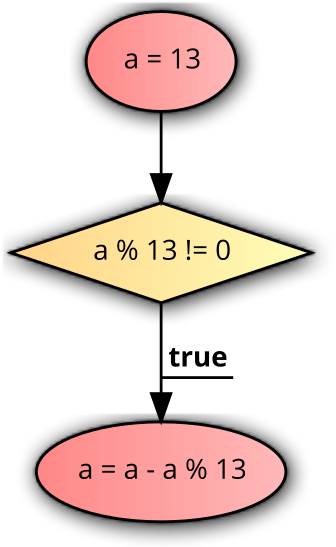
\includegraphics[scale=0.3]{1.png}
\vskip 0.5cm
Program does not result in \textcolor{red}{variable may not be initialized} since all leaves of the flowchart end up in a value being assigned to \texttt{a}.
\end{solution}

\part 
\begin{lstlisting}
int max;
int a = 4, b = 6, c = 2;
if(a >= b && a >= c) {
	max = a;
}
else if(b >= c) {
	max = b;
}
else {
	max = c;
}
\end{lstlisting}

\begin{solution}
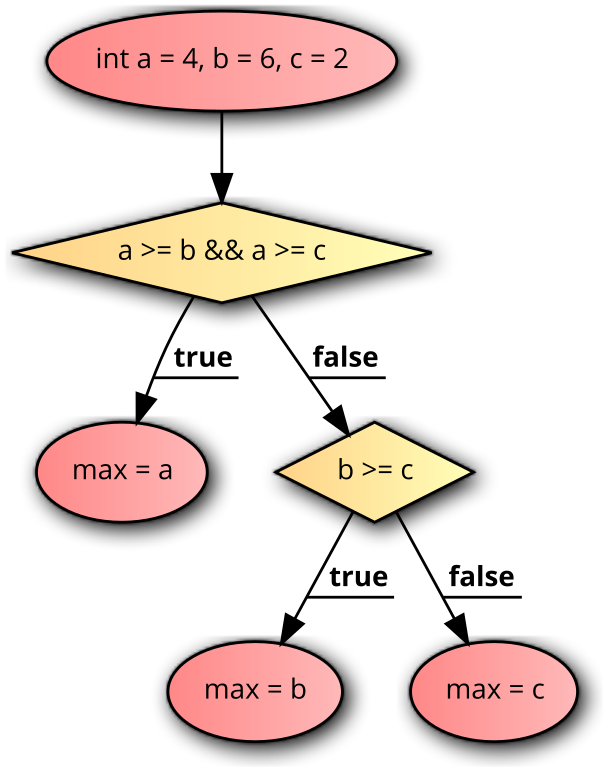
\includegraphics[scale=0.3]{2.png}
\vskip 0.5cm
Program does not result in \textcolor{red}{variable may not be initialized} since all leaves of the flowchart end up in a value being assigned to \texttt{max}.
\end{solution}

\part 
\begin{lstlisting}
boolean sameOddity;
if(a && b) {
	sameOddity = true;
}
if(!a && !b) {
	sameOddity = true;
}
if(a && !b) {
	sameOddity = false;
}
if(!a && b) {
	sameOddity = false;
}
\end{lstlisting}

\begin{solution}
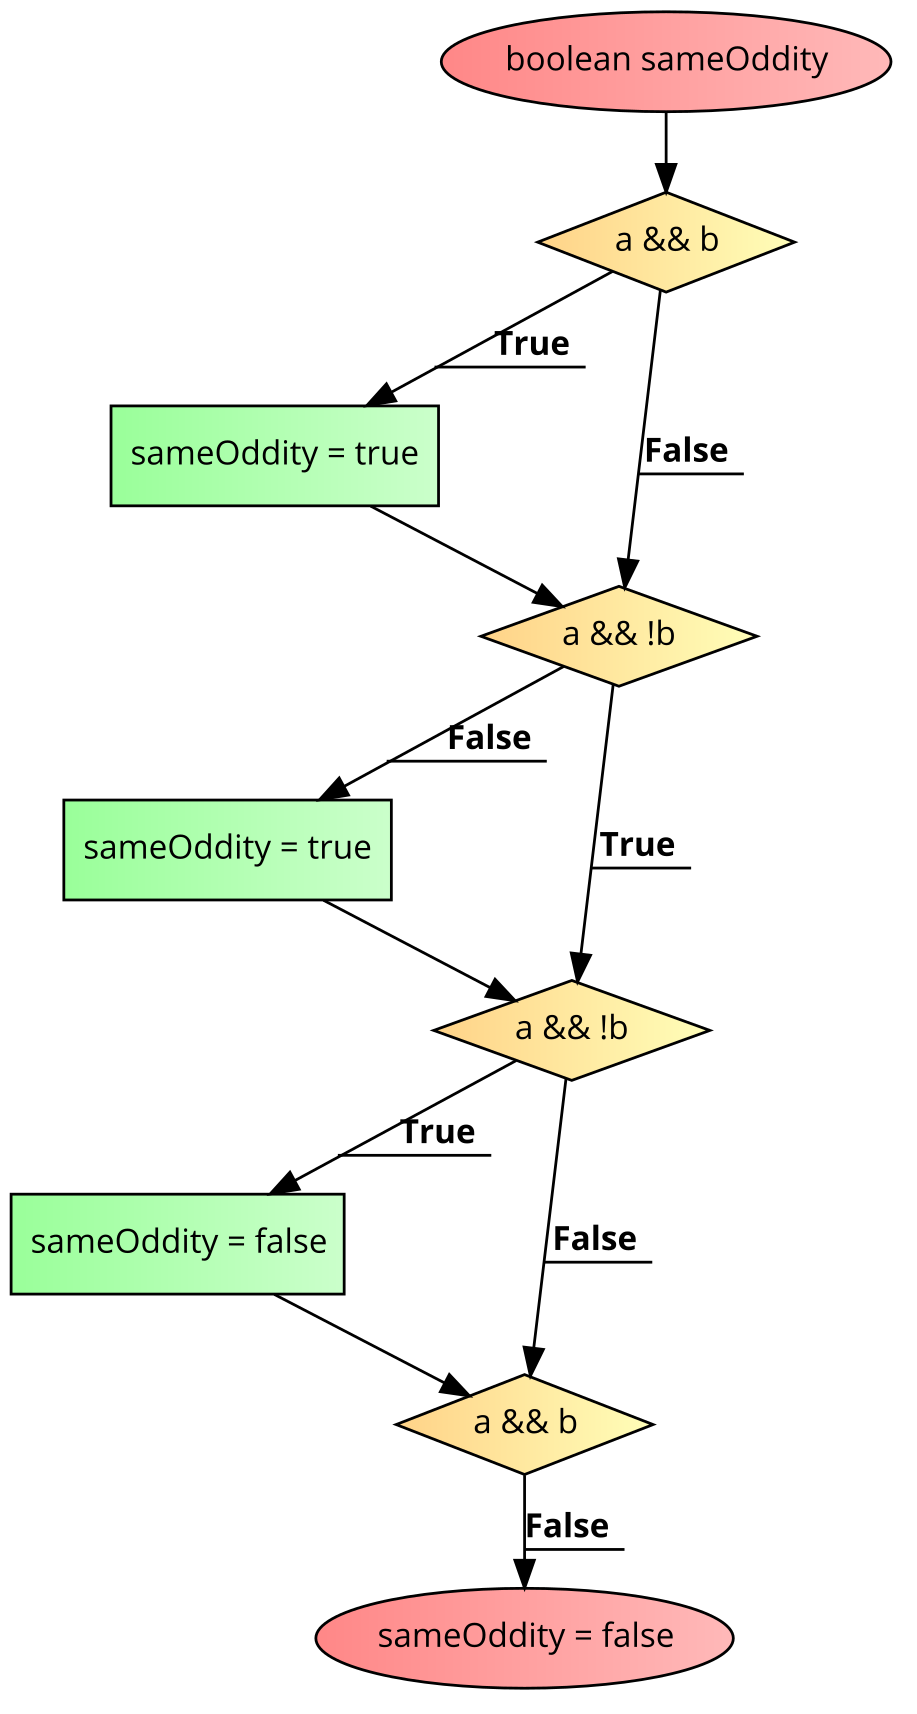
\includegraphics[scale=0.3]{3.png}
\vskip 0.5cm
Program results in \textcolor{red}{variable may not be initialized} since one path of the flowchart end up in a value being assigned to \texttt{sameOddity} (when none of the boolean expressions are true).
\end{solution}
\end{parts}

\question \textbf{Tracing control structures - 1}
Trace the following code and determine the value of result.

\begin{lstlisting}
int a = 114;
int result = 0;
while(a != 0) {
	if(a % 2 == 1) {
		result = result + 1;
	}
	a = a / 2;
}
\end{lstlisting}
\begin{solution}
result = 4 (number of 1s in the binary version of 114)
\end{solution}

\question \textbf{Tracing control structures - 2}
Trace the following code and determine the value of result.

\begin{lstlisting}
int x = 2;
int n = 8;
int result = 1;
for(int i=1; i <= n; i++) {
	result = result * x;
}		
\end{lstlisting}
\begin{solution}
result = 256 (256 = 2 to the power of 8). The program calculates $x^n$.
\end{solution}

\question \textbf{Tracing control structures - 3}
Trace the following code and determine the value of result.

\begin{lstlisting}
int a = 23, b = 49;
int result = 0, power = 1;

while (a != 0 || b != 0) {
  int bit1 = a % 2;
  int bit2 = b % 2;
  if (bit1 != bit2) {
    result = result + power;
  }
  power = power * 2;
  a = a / 2;
  b = b / 2;
}
\end{lstlisting}

\begin{solution}
result = 38	(outcome of a XOR b)
\end{solution}

\question \textbf{Writing control structures - 1}

Consider there are three variables, \texttt{low, high, interval} such that:

\begin{itemize}
	\item \texttt{low} $\leq$ \texttt{high}, and,
	\item \texttt{interval} $\geq 0$
\end{itemize}

Write a piece of code that computes the following value, and stores it in a variable \texttt{sum}.

\begin{verbatim}
low + (low + interval) + (low + 2*interval) + ... high

* note that it might not go all the way to high
\end{verbatim}

For example, 
\begin{verbatim}
low = 3, high = 15, interval = 4 -> sum = 3+7+11+15 = 36
low = 1, high = 8, interval = 5 -> sum = 1+6 = 7
low = -18, high = 20, interval = 12 -> sum = -18+-6+6+18 = 0
\end{verbatim}

\begin{solution}
\begin{lstlisting}
int sum = 0;
for(int i=low; i<=high; i+=interval) {
	sum = sum + i;
}
\end{lstlisting}
\end{solution}

\question \textbf{Writing control structures - 2}

Given an integer $n \geq 1$, write a piece of code that adds  integers from 1 to $n$ with the additional constraints that -

\begin{enumerate}
  \item any multiple of 5 should not be added, unless the number is also a multiple of 10, in which case, we should add twice of that number to the sum.
\end{enumerate}

For example,

\begin{verbatim}
n = 12, sumNot5 = 1+2+3+4+6+7+8+9+2*10+11+12 = 83
\end{verbatim}

\begin{solution}
\begin{lstlisting}
int sumNot5 = 0;
for(int i=1; i<=n; i++) {
	if(i%5 != 0) {
		sumNot5 = sumNot5 + i;
	}
	else if(i%10 == 0) {
		sumNot5 = sumNot5 + 2*i;
	}
}
\end{lstlisting}
\end{solution}

\question \textbf{(ADVANCED) Writing control structures - 3}

In the lecture we discussed how to determine if a given integer is prime or not. The snippet is provided below:

\begin{lstlisting}
boolean isPrime = true;
for(int i=2; i*i<=n && isPrime; i++) {
	if(n%i==0) {
		isPrime = false;
	}
}
\end{lstlisting}

The first few primes are:

\begin{verbatim}
prime 0: 2
prime 1: 3
prime 2: 5
prime 3: 7
prime 4: 11
prime 5: 13
\end{verbatim}
 
(In C-base languages - including Java - we number everything starting at zero).

Given an integer $k \geq 0$, write a piece of code that computes prime $k$.

For example,

\begin{verbatim}
k = 5 -> 13
k = 10 -> 31
k = 45 -> 199
k = 1000 -> 7927
\end{verbatim}

\begin{solution}
\begin{lstlisting}
int n = 2;
int result = n;
if (k > 0) {
  for (int p=0; p<=k; n++) {
    boolean isPrime = true;
    for (int i=2; i*i<=n && isPrime; i++) {
      if (n%i==0) {
        isPrime = false;
      }
    }
    if (isPrime) {
      p++;
    }
  }
  n--; //the last time
}
\end{lstlisting}
\end{solution}

\end{questions}
\end{document}
